\subsection{Determining the Vector Space}
The 4th phase space, succeeding the 3 phase spaces discussed in the lecture, has the following constraints.

\begin{equation}
  \label{equ:constraints}
  \begin{aligned}
    K_1 &> \frac {K_2} {\alpha_1} \\
    K_2 &> \frac {K_1} {\alpha_2}
  \end{aligned}
\end{equation}

This system in a phase space should resemble Figure \ref{fig:graph_001}.

\begin{figure}[h]
  \centering
  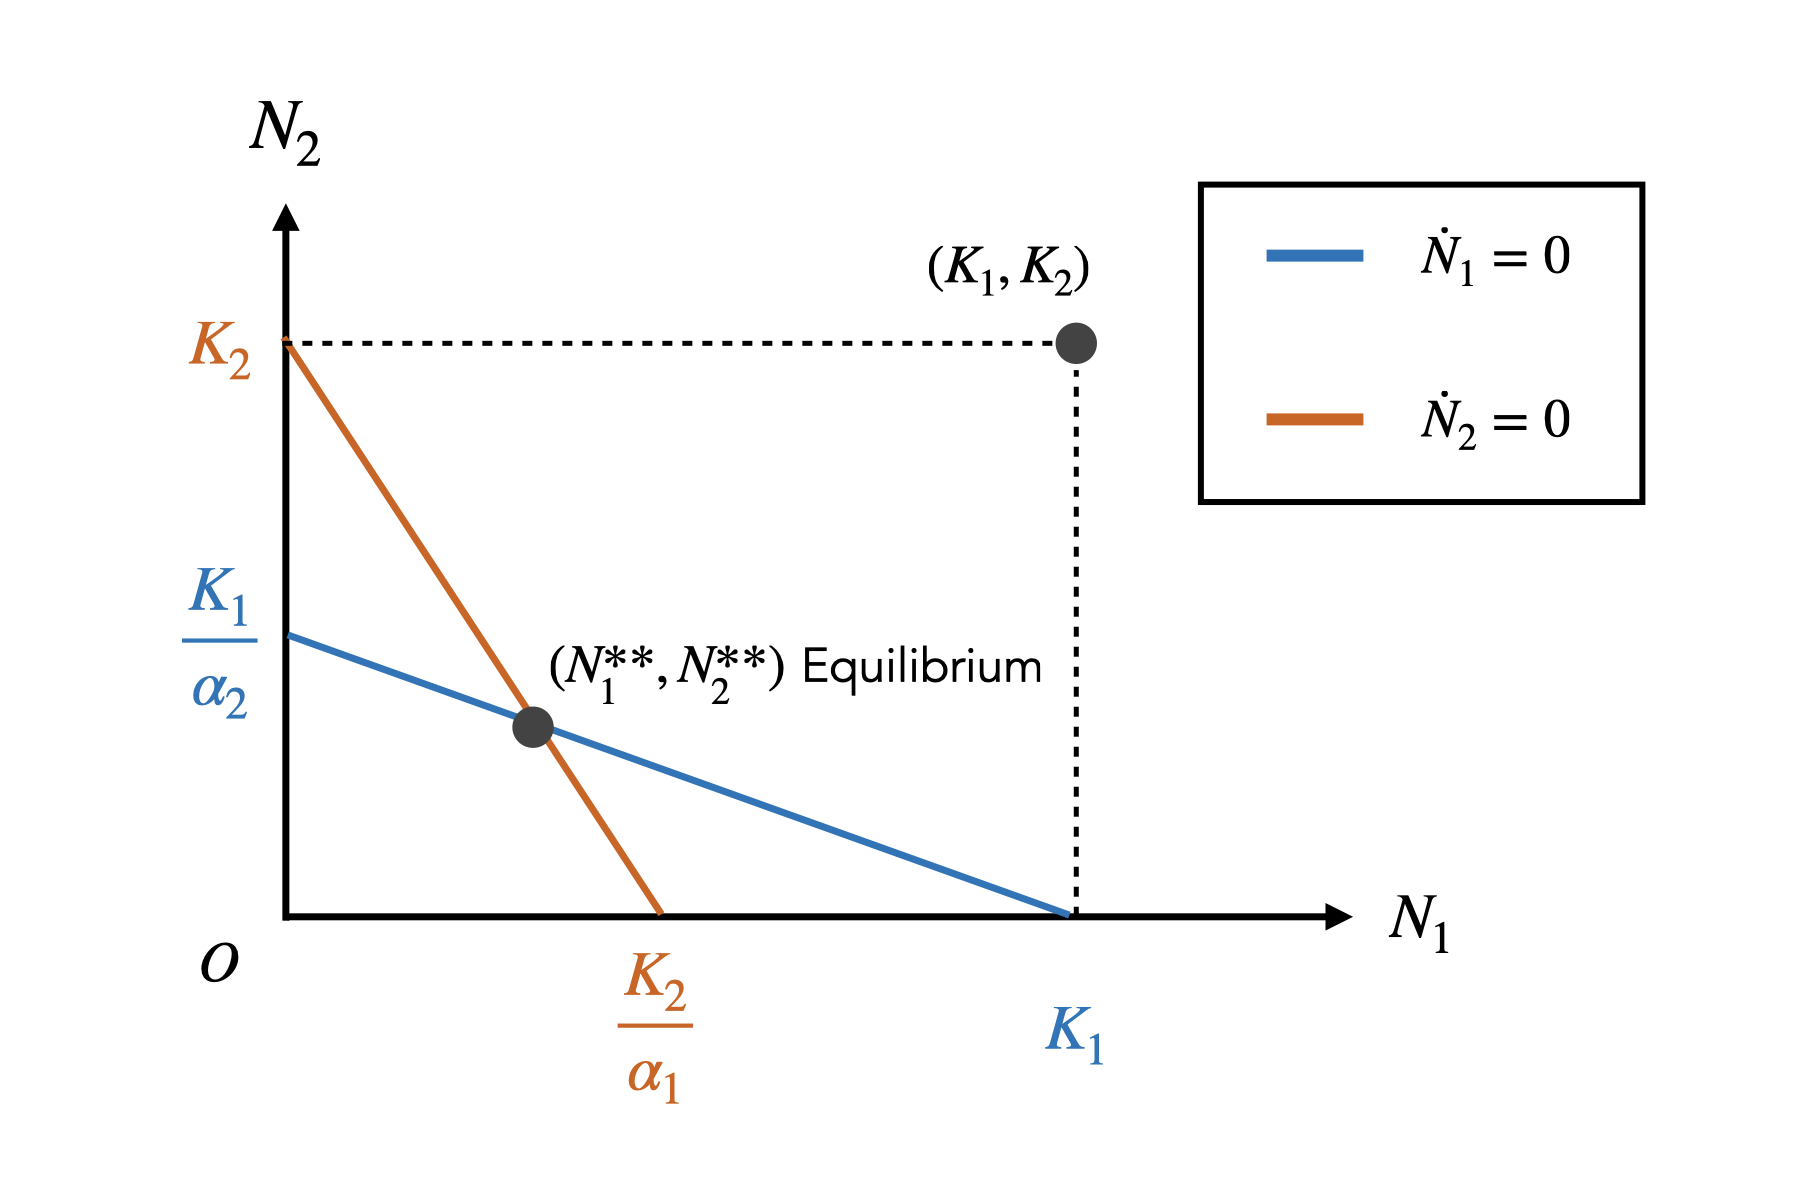
\includegraphics[width = \textwidth]{fig/graph_001.png}
  \caption {Nullclines for $N_1$ and $N_2$ and the equilibrium of the Lotka-Volterra system when Equation \ref{equ:constraints} is met.}
  \label{fig:graph_001}
\end{figure}

In determining the vector space, or rather the vectors' orientation on arbitrary points in the phase plane, we need a sample of a point on the phase plane. For simplicity, we take $(K_1, K_2)$.


Now we determine the orientation of the vector at $(K_1, K_2)$.

\begin{equation}
  \label{equ:dotn1minus}
  \begin{aligned}
    \dot N_1
    &= r_1 N_1 \left( \frac {K_1 - N_1 - \alpha_2 N_2} {K_1} \right) \\
    &= r_1 K_1 \left( \frac {K_1 - K_1 - \alpha_2 N_2} {K_1} \right) \\
    &= - r_1 \alpha_2 K_2 < 0
  \end{aligned}
\end{equation}

\begin{equation}
  \label{equ:dotn2minus}
  \begin{aligned}
    \dot N_2
    &= r_2 N_2 \left( \frac {K_2 - N_2 - \alpha_1 N_1} {K_2} \right) \\
    &= r_2 K_2 \left( \frac {K_2 - K_2 - \alpha_1 N_1} {K_2} \right) \\
    &= - r_2 \alpha_1 K_1 < 0
  \end{aligned}
\end{equation}

Based on Equations \ref{equ:dotn1minus} and \ref{equ:dotn2minus}, we can determine that the vector at $(K_1, K_2)$ is pointed toward the origin.

Given that there are 2 nullclines as specified in \ref{ls:nullclines}, the vector space would look like Figure \ref{fig:vecspace}.

\begin{figure}[h]
  \centering
  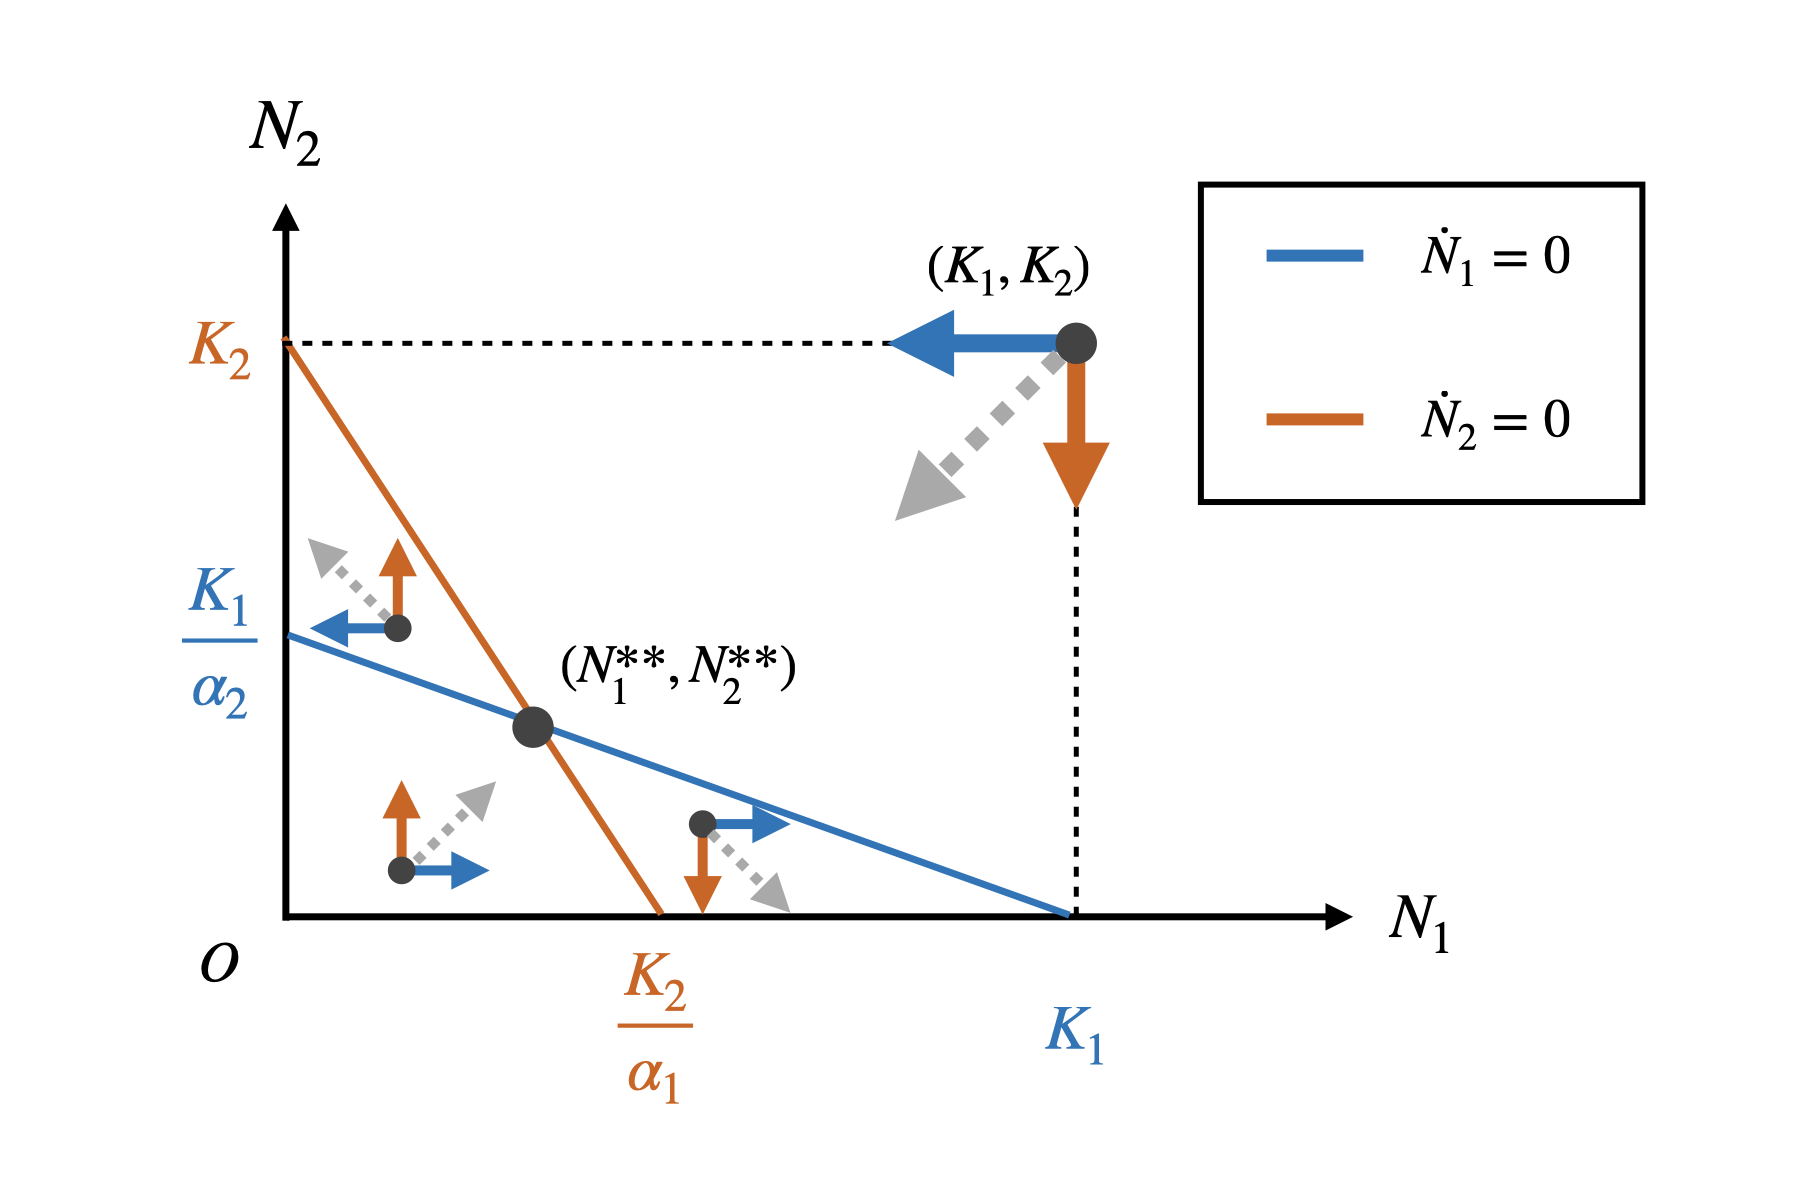
\includegraphics[width = \textwidth]{fig/graph_002.png}
  \caption {Vector space for the Lotka-Volterra model when Equation \ref{equ:constraints} is met. The blue and red arrows indicate the direction of the vector on the $N_1$ and $N_2$ axes per point, respectively. The dotted gray arrows indicate the direction of the vector after combining the previous 2 arrows.}
  \label{fig:vecspace}
\end{figure}
